\chapter{搜索和图论}

用树来展示DFS和BFS的区别如下,其中 $h$ 表示树的深度。可见,DFS在空间上具有更大的优势,而BFS则为指数级别。
\begin{table}[!ht]
    \centering
    \begin{tabular}{|c|c|c|l|}
        \hline
        ~   & 数据结构  & 空间           & ~                        \\ \hline
        DFS & stack & \bigo{$h$}   & 不具有最短性                   \\ \hline
        BFS & queue & \bigo{$2^h$} & 第一次扩展到最近点,最短路性质(边的权重为1时) \\ \hline
    \end{tabular}
\end{table}
可见,因为BFS的最短路性质,当需要解决最小操作数、最短距离、最短路等问题时,可以尝试使用BFS。而当题目难以思考时,可尝试DFS。

稠密图:邻接矩阵 \lstinline{g[N][N]}, a和b之间是否有边,且边的权重是多少

稀疏图:邻接表 \lstinline{h[N], e[N], ne[N], idx}, 和拉链法的哈希是一样的数据结构


\section{DFS}
从搜索树的角度来看,每一个DFS都对应一个搜索树。DFS最重要的是考虑搜索顺序,以什么顺序进行解空间的遍历。

回溯:回溯的过程由递归处理,每次需要手动维护自己的数据结构,保证恢复现场。

剪枝:

\subsection{AcWing 842. 排列数字}
\begin{titledbox}{AcWing 842. 排列数字}
    给定一个整数 $n$,将数字 $1 \sim n$ 排成一排,将会有很多种排列方法。现在,请你按照字典序将所有的排列方法输出。

    输入格式:

    共一行,包含一个整数 $n$。

    输出格式:

    按字典序输出所有排列方案,每个方案占一行。

    数据范围:

    $1 \le n \le 7$

    \begin{inputblock}
        3
    \end{inputblock}
    \begin{outputblock}
        1 2 3 \\
        1 3 2 \\
        2 1 3 \\
        2 3 1 \\
        3 1 2 \\
        3 2 1
    \end{outputblock}
\end{titledbox}

\begin{mycpptwocol}[排列数字]
    #include <stdio.h>
    #include <stdbool.h>

    #define N 10

    int path[N];
    bool st[N];

    void dfs(int u, int n)
        {
        if (u == n) {
            for (int i = 0; i < n; i++) {
                printf("%d ", path[i]);
            }
            printf("\n");
            return;
        }
        for (int i = 1; i <= n; i++) {
            if (!st[i]) {
                path[u] = i;
                st[i] = true;
                dfs(u + 1, n);
                st[i] = false;
            }
        }
    }

    int main()
        {
        int n;
        scanf("%d", &n);
        dfs(0, n);
        return 0;
    }
\end{mycpptwocol}

\subsection{AcWing 843. n-皇后问题}
\begin{titledbox}{AcWing 843. n-皇后问题}
    $n-$皇后问题是指将 $n$ 个皇后放在 $n \times n$ 的国际象棋棋盘上,使得皇后不能相互攻击到,即任意两个皇后都不能处于同一行、同一列或同一斜线上。

    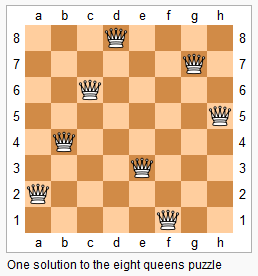
\includegraphics[width=0.3\textwidth]{n-queen.png}

    现在给定整数 $n$,请你输出所有的满足条件的棋子摆法。

    输入格式:

    共一行,包含整数 $n$。

    输出格式:

    每个解决方案占 $n$ 行,每行输出一个长度为 $n$ 的字符串,用来表示完整的棋盘状态。
    其中 \lstinline{.} 表示某一个位置的方格状态为空,\lstinline{Q} 表示某一个位置的方格上摆着皇后。每个方案输出完成后,输出一个空行。\textbf{注意:行末不能有多余空格。}输出方案的顺序任意,只要不重复且没有遗漏即可。

    数据范围:

    $1 \le n \le 9$

    \begin{inputblock}
        4
    \end{inputblock}
    \begin{outputblock}
        .Q.. \\
        ...Q \\
        Q... \\
        ..Q. \\

        ..Q. \\
        Q... \\
        ...Q \\
        .Q..
    \end{outputblock}
\end{titledbox}

有两种解法,第一种:因发现每一行每一列有且仅有一个皇后,可以枚举每一行,来看看可以将皇后放置在第几列。

\begin{mycpptwocol}[n-皇后问题:解法一]
    #include <stdio.h>
    #include <stdlib.h>
    #include <string.h>
    #include <stdbool.h>

    #define N 20

    char g[N][N];
    bool col[N];
    bool dg[N];
    bool udg[N];

    void dfs(int u, int n)
        {
        if (u == n) {
            for (int i = 0; i < n; i++) {
                puts(g[i]);
            }
            printf("\n");
            return;
        }
        for (int i = 0; i < n; i++) {
            if (col[i] || dg[u + i] || udg[u - i + n]) {
                continue;
            }
            g[u][i] = 'Q';
            col[i] = dg[u + i] = udg[u - i + n] = true;
            dfs(u + 1, n);
            g[u][i] = '.';
            col[i] = dg[u + i] = udg[u - i + n] = false;
        }
    }

    int main()
        {
        int n;
        scanf("%d", &n);
        for (int i = 0; i < n; i++) {
            for (int j = 0; j < n; j++) {
                g[i][j] = '.';
            }
        }
        dfs(0,  n);
        return 0;
    }
\end{mycpptwocol}

解法二:从左上角开始枚举每一个格子,每个格子有两种状态(放或者不放),在枚举过程中检查每一个格子是否可以继续放置。若皇后数量已经达到最大数量则找到了一个方案

\begin{mycpptwocol}[n-皇后问题:解法二]
    #include <stdio.h>
    #include <stdlib.h>
    #include <string.h>
    #include <stdbool.h>

    #define N 20

    char g[N][N];
    bool row[N];
    bool col[N];
    bool dg[N];
    bool udg[N];

    void dfs(int x, int y, int s, int n)
        {
        if (y == n) {
            y = 0;
            x++;
        }
        if (x == n) {
            if (s == n) {
                for (int i = 0; i < n; i++) {
                    puts(g[i]);
                }
                puts("");
            }
            return;
        }
        // do not put queen here
        dfs(x, y + 1, s, n);

        // put queen here
        if (!row[x] && !col[y] && !dg[x + y] && !udg[x - y + n]) {
            g[x][y] = 'Q';
            row[x] = col[y] = dg[x + y] = udg[x - y + n] = true;
            dfs(x, y + 1, s + 1, n);
            g[x][y] = '.';
            row[x] = col[y] = dg[x + y] = udg[x - y + n] = false;
        }
    }

    int main()
        {
        int n;
        scanf("%d", &n);
        for (int i = 0; i < n; i++) {
            for (int j = 0; j < n; j++) {
                g[i][j] = '.';
            }
        }
        dfs(0, 0, 0, n);
        return 0;
    }
\end{mycpptwocol}


\section{BFS}

宽度优先搜索的基本思路是初始化一个队列,需要决定队列中存储的是什么。进入队列循环后从对头弹出元素 $t$ 之后,选择 $t$ 可拓展的节点之后将拓展节点入队。

\subsection{AcWing 844. 走迷宫}
\begin{titledbox}{AcWing 844. 走迷宫}
    给定一个 $n \times m$ 的二维整数数组,用来表示一个迷宫,数组中只包含 $0$ 或 $1$,其中 $0$ 表示可以走的路,$1$ 表示不可通过的墙壁。最初,有一个人位于左上角 $(1, 1)$ 处,已知该人每次可以向上、下、左、右任意一个方向移动一个位置。请问,该人从左上角移动至右下角 $(n, m)$ 处,至少需要移动多少次。数据保证 $(1, 1)$ 处和 $(n, m)$ 处的数字为 $0$,且一定至少存在一条通路。

    输入格式:

    第一行包含两个整数 $n$ 和 $m$。接下来 $n$ 行,每行包含 $m$ 个整数($0$ 或 $1$),表示完整的二维数组迷宫。

    输出格式:

    输出一个整数,表示从左上角移动至右下角的最少移动次数。

    数据范围:

    $1 \le n, m \le 100$

    \begin{inputblock}
        5 5 \\
        0 1 0 0 0 \\
        0 1 0 1 0 \\
        0 0 0 0 0 \\
        0 1 1 1 0 \\
        0 0 0 1 0
    \end{inputblock}
    \begin{outputblock}
        8
    \end{outputblock}
\end{titledbox}

\begin{mycpptwocol}[BFS 走迷宫]
    #include <stdio.h>
    #include <stdlib.h>

    #define N 110

    int g[N][N];
    int d[N][N];

    typedef struct {
        int x;
        int y;
    } Pair;

    Pair queue[N * N];

    int bfs(int n, int m)
        {
        int head = 0;
        int tail = 0;
        Pair init = {0, 0};
        queue[tail++] = init;
        memset(d, -1, sizeof(d));
        d[0][0] = 0;

        int dx[4] = {0, 1, 0, -1};
        int dy[4] = {1, 0, -1, 0};

        while (head <= tail) {
            Pair t = queue[head++];
            for (int i = 0; i < 4; i++) {
                int x = t.x + dx[i];
                int y = t.y + dy[i];
                if (x >= 0 && x < n && y >= 0 && y < m && d[x][y] == -1 && g[x][y] == 0) {
                    queue[tail++] = (Pair){x, y};
                    d[x][y] = d[t.x][t.y] + 1;
                }
            }
        }
        return d[n - 1][m - 1];
    }

    int main()
        {
        int n;
        int m;
        scanf("%d %d", &n, &m);
        for (int i = 0; i < n; i++) {
            for (int j = 0; j < m; j++) {
                scanf("%d", &g[i][j]);
            }
        }
        printf("%d", bfs(n, m));
        return 0;
    }
\end{mycpptwocol}

\begin{information}
    若想要输出最短路径,则可以开一个数组 \lstinline{Pair prev[N][N];} 来存储每一个点的前一个节点(在扩展 $t$ 时可以操作),最后从后往前循环输出即可。
\end{information}

\subsection{AcWing 845. 八数码}
\begin{titledbox}{AcWing 845. 八数码}
    在一个 $3 \times 3$ 的网格中,$1 \sim 8$ 这 $8$ 个数字和一个 \lstinline{x} 恰好不重不漏地分布在这 $3 \times 3$ 的网格中。

    例如:

    1 2 3 \\
    x 4 6 \\
    7 5 8

    在游戏过程中,可以把 \lstinline{x} 与其上、下、左、右四个方向之一的数字交换(如果存在)。
    我们的目的是通过交换,使得网格变为如下排列(称为正确排列):

    1 2 3 \\
    4 5 6 \\
    7 8 x

    例如,示例中图形就可以通过让 \lstinline{x} 先后与右、下、右三个方向的数字交换成功得到正确排列。
    交换过程如下:

    1 2 3 \hspace{1em} 1 2 3 \hspace{1em} 1 2 3 \hspace{1em} 1 2 3 \\
    x 4 6 \hspace{1em} 4 x 6 \hspace{1em} 4 5 6 \hspace{1em} 4 5 6 \\
    7 5 8 \hspace{1em} 7 5 8 \hspace{1em} 7 x 8 \hspace{1em} 7 8 x

    现在,给你一个初始网格,请你求出得到正确排列至少需要进行多少次交换。

    输入格式:

    输入占一行,将 $3 \times 3$ 的初始网格描绘出来。例如,如果初始网格如下所示:

    1 2 3 \\
    x 4 6 \\
    7 5 8

    则输入为:\lstinline{1 2 3 x 4 6 7 5 8}

    输出格式:

    输出占一行,包含一个整数,表示最少交换次数。如果不存在解决方案,则输出 $-1$。

    \begin{inputblock}
        2 3 4 1 5 x 7 6 8
    \end{inputblock}
    \begin{outputblock}
        19
    \end{outputblock}
\end{titledbox}


\section{树与图的存储}
树是一种特殊的图(无环联通图);图分为有向图和无向图,无向图又可看作是特殊的有向图(每两个相连的节点之间有两条分别指向对方的边)。所以树和图均可统一看作图,故此处仅讨论有向图的存储方式。

有向图的存储有两种方式:
\begin{description}
    \item[邻接矩阵]
    使用二维数组存储图 \lstinline{g[a][b]} 表示边 $a \rightarrow b$ 上的权重,若无权图则表示边的存在性。空间复杂度为 \bigo{$n^2$} ,比较浪费空间,常用来存储稠密图。
    \item[邻接表]
    使用链表的形式,每一个节点对应一个单链表来存储由该点出发可以走到的所有点。
\end{description}
由上可见,邻接表的存储方式和Hash表的拉链法是一样的。


\section{树与图的深度优先遍历}

模版如下:
\begin{mycpptwocol}[dfs in tree and graphic]
    int h[N], e[M], ne[M], idx;
    bool st[N]; // 状态数组,存储节点时候已访问

    void add(int a, int b) {
        e[++idx] = b;
        ne[idx] = h[a];
        h[a] = idx;
    }

    void dfs(int u) {
        st[u] = true;
        for (int i = h[t]; i != -1; i = ne[i]) {
            int j = e[i];
            if (!st[j] && check(j)) {
                dfs(j);
            }
        }
    }
\end{mycpptwocol}
其中,14行的 \lstinline{check(j)} 的作用是剪枝。

\subsection{AcWing 846. 树的重心}
\begin{titledbox}{AcWing 846. 树的重心}
    给定一棵树,树中包含 $n$ 个结点(编号 $1 \sim n$)和 $n-1$ 条无向边。请你找到树的重心,并输出将重心删除后,剩余各个连通块中点数的最大值。

    重心定义:重心是指树中的一个结点,如果将这个点删除后,剩余各个连通块中点数的最大值最小,那么这个节点被称为树的重心。

    输入格式:

    第一行包含整数 $n$,表示树的结点数。接下来 $n-1$ 行,每行包含两个整数 $a$ 和 $b$,表示点 $a$ 和点 $b$ 之间存在一条边。

    输出格式:

    输出一个整数 $m$,表示将重心删除后,剩余各个连通块中点数的最大值。

    数据范围:

    $1 \le n \le 10^5$

    \begin{inputblock}
        9 \\
        1 2 \\
        1 7 \\
        1 4 \\
        2 8 \\
        2 5 \\
        4 3 \\
        3 9 \\
        4 6
    \end{inputblock}
    \begin{outputblock}
        4
    \end{outputblock}
\end{titledbox}

\begin{mycpptwocol}[树的DFS]
    #include <stdio.h>
    #include <stdlib.h>
    #include <stdbool.h>

    #define N 100010

    int h[N], e[N], ne[N], idx;
    bool st[N];
    int ans = N;

    void add(int a, int b) {
        e[++idx] = b;
        ne[idx] = h[a];
        h[a] = idx;
    }

    int max(int a, int b) {
        return a > b ? a : b;
    }

    int min(int a, int b) {
        return a < b ? a : b;
    }

    // 返回以节点u为根的子树的节点数
    int dfs(int u, int n) {
        st[u] = true;

        int sum = 1; // 计入当前节点
        // res为去掉u之后所有连通块中节点数最大值
        int res = 0;
        for (int i = h[u]; i != -1; i = ne[i]) {
            int j = e[i];
            if (!st[j]) {
                int s = dfs(j, n);
                res = max(res, s);
                sum += s;
            }
        }
        res = max(res, n - sum);
        ans = min(ans, res);
        return sum;
    }

    int main() {
        memset(h, -1, sizeof(h));
        int n;
        scanf("%d", &n);

        int a;
        int b;
        for (int i = 0; i < n - 1; i++) {
            scanf("%d %d", &a, &b);
            add(a, b);
            add(b, a);
        }
        dfs(1, n);
        printf("%d", ans);
        return 0;
    }
\end{mycpptwocol}


\section{树与图的广度优先遍历}

\subsection{AcWing 847. 图中点的层次}
\begin{titledbox}{AcWing 847. 图中点的层次}
    给定一个 $n$ 个点 $m$ 条边的有向图,图中可能存在重边和自环。所有边的长度都是 $1$,点的编号为 $1 \sim n$。请你求出 $1$ 号点到 $n$ 号点的最短距离,如果从 $1$ 号点无法走到 $n$ 号点,输出 $-1$。

    输入格式:

    第一行包含两个整数 $n$ 和 $m$。接下来 $m$ 行,每行包含两个整数 $a$ 和 $b$,表示存在一条从 $a$ 走到 $b$ 的长度为 $1$ 的边。

    输出格式:

    输出一个整数,表示 $1$ 号点到 $n$ 号点的最短距离。

    数据范围:

    $1 \le n,m \le 10^5$

    \begin{inputblock}
        4 5 \\
        1 2 \\
        2 3 \\
        3 4 \\
        1 3 \\
        1 4
    \end{inputblock}
    \begin{outputblock}
        1
    \end{outputblock}
\end{titledbox}

\begin{mycpptwocol}[图的BFS]
    #include <stdio.h>
    #include <stdlib.h>

    #define N 100010

    int h[N], e[N], ne[N], idx;

    int d[N];

    void add(int a, int b) {
        e[++idx] = b;
        ne[idx] = h[a];
        h[a] = idx;
    }

    int bfs(int n) {
        int *q = (int *)calloc(n, sizeof(int));
        int tt = 0;
        int hh = 0;
        q[tt++] = 1;
        d[1] = 0;
        while (hh < tt) {
            int t = q[hh++];
            for (int i = h[t]; i != -1; i = ne[i]) {
                int j = e[i];
                if (d[j] == -1) {
                    d[j] = d[t] + 1;
                    q[tt++] = j;
                }
            }
        }
        return d[n];
    }

    int main() {
        memset(h, -1, sizeof(h));
        memset(d, -1, sizeof(d));
        int n;
        int m;
        scanf("%d %d", &n, &m);
        int a;
        int b;
        while (m--) {
            scanf("%d %d", &a, &b);
            add(a, b);
        }
        printf("%d", bfs(n));
        return 0;
    }
\end{mycpptwocol}


\section{拓扑排序}

\subsection{AcWing 848. 有向图的拓扑序列}
\begin{titledbox}{AcWing 848. 有向图的拓扑序列}
    给定一个 $n$ 个点 $m$ 条边的有向图,点的编号是 $1$ 到 $n$,图中可能存在重边和自环。请输出任意一个该有向图的拓扑序列,如果拓扑序列不存在,则输出 $-1$。若一个由图中所有点构成的序列 $A$ 满足:对于图中的每条边 $(x, y)$,$x$ 在 $A$ 中都出现在 $y$ 之前,则称 $A$ 是该图的一个拓扑序列。

    输入格式:

    第一行包含两个整数 $n$ 和 $m$。接下来 $m$ 行,每行包含两个整数 $x$ 和 $y$,表示存在一条从点 $x$ 到点 $y$ 的有向边 $(x, y)$。

    输出格式:

    共一行,如果存在拓扑序列,则输出任意一个合法的拓扑序列即可。否则输出 $-1$。

    数据范围:

    $1 \le n,m \le 10^5$

    \begin{inputblock}
        3 3 \\
        1 2 \\
        2 3 \\
        1 3 \\
    \end{inputblock}
    \begin{outputblock}
        1 2 3
    \end{outputblock}
\end{titledbox}

\begin{mycpptwocol}[拓扑排序]
    #include <stdio.h>
    #include <stdlib.h>
    #include <stdbool.h>

    #define N 100010

    int h[N], e[N], ne[N], idx;
    int degree[N];

    int q[N], hh, tt;

    void Add(int a, int b) {
        e[++idx] = b;
        ne[idx] = h[a];
        h[a] = idx;
        degree[b]++;
    }

    bool TopoSort(int n) {
        for (int i = 1; i <= n; i++) {
            if (degree[i] == 0) {
                q[tt++] = i;
            }
        }
        while (hh < tt) {
            int t = q[hh++];
            for (int i = h[t]; i != -1; i = ne[i]) {
                int j = e[i];
                degree[j]--;
                if (degree[j] == 0) {
                    q[tt++] = j;
                }
            }
        }
        return tt == n;
    }

    int main()
        {
        memset(h, -1, sizeof(h));
        int n;
        int m;
        scanf("%d %d", &n, &m);
        int a;
        int b;
        while (m--) {
            scanf("%d %d", &a, &b);
            Add(a, b);
        }
        if (TopoSort(n)) {
            int hh = 0;
            while (hh < tt) {
                printf("%d ", q[hh++]);
            }
        } else {
            puts("-1");
        }
        return 0;
    }
\end{mycpptwocol}


\section{有向图的最短路问题}
这一节将关注在图的最短路的求解上,最短路问题及其常见方法如下:

最短路问题:$n$ 表示点数,$m$ 表示边数

\begin{enumerate}
    \item 单源最短路:求一个点到其他所有点的最短路
    \begin{itemize}
        \item 所有边权都是正数:1. 朴素dijkstra算法\bigo{$n^2$},与边数无关,适合稠密图 2. 堆优化版的dijkstra算法 \bigo{$m\log{}n$} 稀疏图:$m$ 与 $n$ 量级相同
        \item 存在负权边:1. Bellman-Ford算法 \bigo{$nm$} 2. SPFA \bigo{$m$}最坏 \bigo{$nm$}
    \end{itemize}
    \item 多源汇最短路:起点和终点不确定,问 $a$ 到 $b$ 的最短路
    \begin{itemize}
        \item Floyd算法 \bigo{$n^3$}
    \end{itemize}
\end{enumerate}

\subsection{AcWing 849. Dijkstra求最短路 I}

朴素版的Dijkstra算法:

1. 用邻接矩阵存储图;\lstinline{g[N][N]}

2. 用一个数组存储每一个点到起始点的距离\lstinline{d[N]};

3. \lstinline{st[N]},存储每一个点是否已经找到了最短路

算法逻辑:

1. 将距离数组初始化为\lstinline{d[i] = +∞; d[k] = 0;} $k$ 表示起始点

2. 从第$0$个点到第$n - 1$个点,找到距离当前点最近的下一个点(遍历$1 - n$) \lstinline{}{t; st[t] = true;}

3. 用$t$更新其他点的距离(遍历$1 - n$)


\begin{titledbox}{AcWing 849. Dijkstra求最短路 I}
    给定一个 $n$ 个点 $m$ 条边的有向图,图中可能存在重边和自环,所有边权均为正值。请你求出 $1$ 号点到 $n$ 号点的最短距离,如果无法从 $1$ 号点走到 $n$ 号点,则输出 $-1$。

    输入格式:

    第一行包含整数 $n$ 和 $m$。接下来 $m$ 行每行包含三个整数 $x,y,z$,表示存在一条从点 $x$ 到点 $y$ 的有向边,边长为 $z$。

    输出格式:

    输出一个整数,表示 $1$ 号点到 $n$ 号点的最短距离。如果路径不存在,则输出 $-1$。

    数据范围:

    $1 \le n \le 500$, $1 \le m \le 10^5$,图中涉及边长均不超过10000。

    \begin{inputblock}
        3 3 \\
        1 2 2 \\
        2 3 1 \\
        1 3 4
    \end{inputblock}
    \begin{outputblock}
        3
    \end{outputblock}
\end{titledbox}

\subsection{AcWing 850. Dijkstra求最短路 II}

注意到在朴素版的Dijkstra算法中需要找到当前节点之后的所有节点中距离最小的那个点的复杂度是 \bigo{$n$},而堆中寻找最小值的复杂度则为 \bigo{$1$}。所以可以用堆来优化这个过程。后面用到了修改堆中元素,为了简单起见,直接插入即可。

如果稠密图中 $n$ 的量为 $10^5$ 时 \bigo{$n^2$} 将会超时,所以选择使用堆对其进行优化,将其降低到 \bigo{$m \log{}n$}

\begin{titledbox}{AcWing 850. Dijkstra求最短路 II}
    给定一个 $n$ 个点 $m$ 条边的有向图,图中可能存在重边和自环,所有边权均为正值。请你求出 $1$ 号点到 $n$ 号点的最短距离,如果无法从 $1$ 号点走到 $n$ 号点,则输出 $-1$。

    输入格式:

    第一行包含整数 $n$ 和 $m$。接下来 $m$ 行每行包含三个整数 $x,y,z$,表示存在一条从点 $x$ 到点 $y$ 的有向边,边长为 $z$。

    输出格式:

    输出一个整数,表示 $1$ 号点到 $n$ 号点的最短距离。如果路径不存在,则输出 $-1$。

    数据范围:

    $1 \le n, m \le 1.5 \times 10^5$,图中涉及边长均不小于 0,且不超过 10000。

    \begin{inputblock}
        3 3 \\
        1 2 2 \\
        2 3 1 \\
        1 3 4
    \end{inputblock}
    \begin{outputblock}
        3
    \end{outputblock}
\end{titledbox}

\subsection{bellman-ford}
处理有负权边的图,如果有负权回路的话最短路不一定存在。所以一般不能有负权回路。

算法逻辑:

1. 循环n个点

2. 循环所有边 \lstinline{a, b, w: dist[b] = min(dist[b], dist[a] + w)} 更新所有距离

因为算法特点存储图时不必使用邻接矩阵或者邻接表,开一个结构体数组:

\begin{mycpponecol}[边集]
    struct {
        int a;
        int b;
        int w;
    } Edges[N]
\end{mycpponecol}

只要能够遍历到所有边即可。可以证明,该算法完成后一定有\textbf{三角不等式}:\lstinline{dist[b] <= dist[a] + w}成立
更新距离数组的过程叫做\textbf{松弛操作}。

第一个循环中,如果当前迭代了 $k$ 次,此时的 \lstinline{dist} 数组表示的是从$1$号点经过不超过$k$条边走到每个点的距离,所以可以用这个原理来找负环,迭代到第 $n$ 次仍能更新则表示有 $n+1$ 个点,但实际只有 $n$ 个点,所以一定存在负环。但一般不用该算法找负环。

\subsection{AcWing 853. 有边数限制的最短路}

\subsection{spfa}
spfa算法是对bellman-ford算法的优化,在松弛操作中,不一定每一次都会对该点的距离减小有所贡献,只有与之相连的前驱节点距离减小了,此时才有可能有所贡献。

用一个bfs来做优化,队列中存储所有变小了距离的节点

\subsection{AcWing 851. spfa求最短路}

\subsection{AcWing 852. spfa判断负环}

\subsection{Floyd}
求多源汇最短路,用邻接矩阵来存储 \lstinline{d[i, j]}

\begin{mycpponecol}[Floyd算法]
    for (int k = 1; k <= n; ++k) {
        for (int i = 1; i <= n; ++i) {
            for (int j = 1; j <= n; ++j) {
                d[i, j] = min(d[i, j], d[i, k] + d[k, j]);
            }
        }
    }
\end{mycpponecol}

初始时, \lstinline{d[i, j]} 就是邻接矩阵,结束之后 \lstinline{d[i, j]} 是最短路长度

\subsection{AcWing 854. Floyd求最短路}


\section{无向图的最小生成树问题}

1. 普里姆算法(Prim算法)1. 朴素版Prim(稠密图)\bigo{$n^2$} 2.堆优化版Prim(稀疏图)\bigo{$m\log{} n$},一般用不到

2. 克鲁斯卡尔算法(Kruskal算法)\bigo{$m\log{} m$} 稀疏图

\subsection{AcWing 858. Prim算法求最小生成树}
Prim算法,与dijkstra算法类似:

Prim算法:

1. 用邻接矩阵存储图;\lstinline{g[N][N]}

2. 用一个数组存储每一个点到集合的距离 \lstinline{d[N]}, 即存储该点所连接边的最小权重;

3. 集合 \lstinline{st[N]},存储当前已经在连通块中的点

算法逻辑:

1. 将距离数组初始化为 \lstinline{d[i] = +∞; d[0] = 1;}

2. 从第 $0$ 个点到第 $n - 1$ 个点,找到集合外距离最近的点 \lstinline{t; st[t] = true;}

3. 用 $t$ 更新其他点到集合的距离

\subsection{AcWing 859. Kruskal算法求最小生成树}

1. 将所有边按照权重从小到大排序;\bigo{$m\log{} m$}

2. 枚举每条边 $a$, $b$, 权重 $c$,如果 $a$ 和 $b$ 不连通,就把这条边加入到集合中。并查集


\section{二分图}

定义:一个图的所有节点可以划分到两个集合中使得图中的边都只存在于集合之间的图称其为可二分的图。

性质:一个图是二分图,当且仅当一个图可以被二染色,当且仅当图中没有奇数环(环中边个数为奇数)

1. 染色法 \bigo{$n + m$}

2. 匈牙利算法 最坏 \bigo{$mn$}, 实际运行时间一般远小于 \bigo{$mn$}

\subsection{AcWing 860. 染色法判定二分图}

\subsection{匈牙利算法}

\subsection{AcWing 861. 二分图的最大匹配}
